\documentclass[11pt, a4paper]{report}
\usepackage[utf8]{inputenc}                             % Encode input with UTF8
\usepackage[T1]{fontenc}                                % Encode output with T1
\usepackage{lmodern}                                    % Force Computer Modern
\usepackage{a4wide}
%\usepackage[margin=2.5cm]{geometry}                     % Specify margin
\usepackage{url}                                        % Allow URLs
\usepackage{color,hyperref}                             % Hyperlink and colour customization
\usepackage{graphicx}                                   % Allow images
\usepackage{booktabs}                                   % Snazzy tables
\usepackage{pdfpages}
\usepackage[section]{placeins}
\usepackage[parfill]{parskip}
%\usepackage[titletoc,title]{appendix}

%\setcounter{secnumdepth}{0}                             % Manual section numbering
%\setlength{\parindent}{0pt}                             % No paragraph indentation

% Customize the URL colouring
\definecolor{darkblue}{rgb}{0.0,0.0,0.3} 		%dette er tull
\hypersetup{colorlinks,
            breaklinks,
            linkcolor=darkblue,
            urlcolor=darkblue,
            anchorcolor=darkblue,
            citecolor=darkblue
}

% PDF metadata
\hypersetup{pdftitle={Process Report Group 2 Experts in team},
            pdfauthor={Eirik Skjeggestad Dale, Hanne Thorshaug Andresen, Marius Ekerholt, Børge Irgens, Leif-Einar H. Pettersen, Hallstein Skjølsvik},
            pdfkeywords={EiT, Process},
}


% BEGIN DOCUMENT
\begin{document}

% TITLE PAGE
\begin{titlepage}
\begin{center}

\vspace*{6cm}
{\Huge TFE4850 - EiT - Student satelite}

\vspace*{0.5cm}
{\LARGE\textbf{Bluebox}}

\vspace*{0.7cm}
{\Large
	Eirik Skjeggestad Dale\\
	Hanne Thorshaug Andresen\\
	Marius Ekerholt\\
	Børge Irgens\\
	Leif-Einar H. Pettersen\\
	Hallstein Skjølsvik
}

{\vfill\textbf{\today}}

\end{center}
\end{titlepage}

\section*{Abstract}

This report is a part of the result of Experts in Teamwork village TFE4850 Student Satellite, spring 2013. EiT is a interdisciplinary course, where the students from different study programs work together to acheieve a common goal. It is important to use the different knowledge in constructiv manner and work well together under pressure to achiece effectivity and reach our goal. 

An important part of this course is to focus on how the group work together and communicates internally. This is a report that describes this process, and we emphasize individual situations which we believe has been of great importance to the group collaboration. We have focused on using relevant theory and joint reflection to create an understanding of what happened,  what we could have done differently and how to improve the process on this basis. We will also try to locate patterns of behavior that affects the group work. 

Our project has the problem definition "Examine the possibility and usefulness of a groundstation network with emphasis on Carpcomm" (bare skrev noe her). We have tried to connect the ground station at NTNU up to Carpcom Space Newtwork and investegated whether this is profitable and possible. 




\section*{Preface}

This report is a part of the result of the Experts in Teamwork village TFE4850 Student Satellite, spring 2013. EiT is a interdisciplinary course, where students from different study programs work together to achieve a common goal. It is important to use the different knowledge in constructive manner and work well together under pressure to achieve effectiveness and reach our goal. 

An important part of this course is to focus on how the group work together and communicates internally. This is a report that describes this process, and we emphasize individual situations which we believe has been of great importance to the group collaboration. We have focused on using relevant theory and joint reflection to create an understanding of what happened,  what we could have done differently and how to improve the process on this basis. We will also try to locate patterns of behavior that affects the group work. 







% TABLE OF CONTENTS
\tableofcontents

% LIST OF FIGURES
%\listoffigures

% LIST OF TABLES
%\listoftables

% THE ACTUAL CONTENTS
\chapter{Introduction}
\label{chap:introduction}
This chapter will contain a short introduction to our project. That means what we're doing and what people are working on the project. It will also be discussed some short background on why we're doing this project.
\section{The Project group}
The project group consisted of 6 people from 5 different institutes, so we have competency in a variety of fields. The group members can be seen in \autoref{tab:groupmembers}.

\begin{table}
	\begin{center}
		\begin{tabular}{|l|l|}   
			\hline      
			\bf{Name} & \bf{Background} \\ 
			\hline
			Marius Ekerholt & Computer technology\\     
			\hline
			Eirik Skjeggestad Dale & Computer technology\\     
			\hline
			Hanne Thorshaug Andresen & Energy and Environmental technology\\     
			\hline
			Leif-Einar H. Pettersen & Electronics and Telecommunications\\     
			\hline
			Børge Irgens & Theoretical Physics\\     
			\hline
			Hallstein Skjølsvik & Electronics and digital design\\     
			\hline
		 \end{tabular}
	\end{center}
	\caption{Group members}
	\label{tab:groupmembers}
\end{table}

\section{Network}

The problem today is that the transfer rate for a satelite using amateur radio is low and the the number of pases are limited. We wanted to look more into this problem and find a solution. Since the transfer rate is limited by the antenna its hard to increase the transferrate without changing the antenna itself. We therefore chose to dive more into how we could increase the number of downstream per pas. We looked into how we could utilize a network of ground stations. We needed to find an existing network that had other ground stations already connected. Carpcomm had seemingly a well established network and was one of the main reason for why we chose it.

\section{NUTS}

NUTS is a student driven satellite project at NTNU. The goal of the project is to design and build a double Cubesat. The student satellite project is organized under the  Department of Electronics and Telecommunications. 
\chapter{The Process}
This chapter contains what we did during the project in terms of the team process. We will discuss the different process elements used and how it affected the group, and helped us improve our teamwork process.
\section{Teamwork agreement}
Something useful about sammarbeidsavtalen.
\section{The Sosiogram}
During the project the facilitators went around to the groups, analyzing the communication flow within the team during a discussion. They made a sosiogram of it by drawing lines to represent whenever someone talked to individuals or the group as a whole, as we can see in the sosiogram from our group, seen in \autoref{fig:sosiogram}. This sosiogram was made while we had one of our mid-day meetings. None of the group members knew that they were being facilitated. Note that when someone talked to the group in general, it's represented as a line towards the center dot of the "table".

The sosiogram showed that the communication flow had broken down, i.e. some people were hardly involved in the discussion at all, and this was a surprise to us. Hanne, one of the most active participants, was surprised she did not notice that Eirik and Marius were not participating in the discussion, as she had felt that all the members were contributing. Marius was one of the members focused on doing research on the computer while the group was meeting. He was also surprised over the sociogram because he felt that he could do research and contribute in the group meeting at the same time. On the contrary the sosiogram shows that the members that had their computers up were almost absent from the discussion.

One of the big advantages of a group project is that you get different points of view and constructive criticism of your ideas, so this is something we did not want. Since the sociogram showed that everyone was about as active as the others, with exception of those using their laptop, we decided to add a norm saying that from now on every meeting shall be pc-free, with the exception of the secretary. 

We managed to keep this norm for the rest of the project and we felt that it improved our creativity and productivity. It is hard to measure, but one thing we noticed was that we did not have to repeat the same topics that had been discussed earlier because all group members paid attention and focused on the meeting. 

%The interesting thing about this sosiogram was that all the group members were surprised by how the communication flow had broken down, i.e. some people were far more active in the discussion than others. The group tried to analyse why this had happened and we believe that this was caused by Eirik and Marius having their computers up. The computers first came up to find some information for the discussion, but stayed up longer than necessary and were a distraction.
%Hanne was one of the most active in the group. She was surprised that she didn't notice that  Marius and Erik wasn’t participating in the discussion. She felt that all members were contributing. Marius was one of the members that were focused on doing research on the computer while the group had a meeting. He was also surprised over the sociogram because he felt that he could do research at the same time as contributing in the group meeting. 

%From the sociogram the group reached the conclusion that the two people sitting on their laptop during the meeting, even though they were doing work relevant for the project, was much less active in the discussion. Since one of the big advantages of a group project is that you get different points of view and can have a discussion about the subject the group decided that this was something we didn't want. We wanted to see the effect of interdisciplinary backgrounds. Since the sociogram showed that everyone was about as active as the others, with exception of those using their laptop , we decided to add a norm saying that from now on every meeting shall be pc-free, unless someone was specifically asked to either take notes as a secretary, or check something that we would need in the discussion.

%We managed to keep this norm for the rest of the project and we felt that it improved our creativity and productivity. It is hard to measure it, but the thing we noticed was that we didn't have to repeat the same topics that had been discussed earlier because all group members paid attention and focused on the meeting. 
\begin{figure}
	\begin{center}
		\includegraphics[trim = 10mm 10mm 10mm 250mm, clip, width=0.7\textwidth]{Figures/sosiogram.png}
	\end{center}
	\caption[The Sosiogram]{The Sosiogram we got from the facilitators after they observed a discussion in the group}
	\label{fig:sosiogram}
\end{figure}
\section{February 13, Changing project definition}

During our project we met some obstacles, which made us, change our project definition. We want to emphasis this day since we feel it represent how our group handles setbacks.

When we started our project we had decided on one type of ground station network that we wanted to test and use. We had spent some time exploring the BlueBox network and every group member had done research. We learned that we were dependent on external partners to complete and work with our project, but were optimistic that we would get the information we needed. We where surprised when we got the news that Aalborg University did not have the opportunity to provide us with the needed information about BlueBox. Hallstein and Leif-Arne who had put in a lot of time understanding some of the technical aspects of BlueBox, felt that they had worked in vain and lost their motivation. As Weeland describes the fundamental attribution error \cite{EffectiveTeamMembers} we started blaming others for our defeat. Thoughts along the lines: "Its the Aalborg Universities fault that we have to start from the beginning, why would they not give us any help?" and " Its not our fault!" surfaced among different team members. 

As the motivation went down we all became ineffective and unproductive. But putting the blame on others would not help us get any further with our project. We took Weelands advice and started finding the factors that was blocking the group progress. By not blaming "the other guy", and remembering that all group members have responsibility for the group's successes and failures we became more motivated to put in a good effort every day. 

As a group we wanted to focus on creating an effective group, high-performance group, by following Schwartz ground rule nine \cite{EffectiveGroups}, which details decision making. We had earlier decided to have a flat structure within the group, without any appointed leader, and a democratic decision-making process \cite{EffectiveGroups}. This time we would ensure that the project was feasible, and used ground rule two. This rule stated that each member share all the relevant information she or he has that affects how the group solves a problem or makes a decision. We then put up a checklist over other ground station network that could be a solution for us. Every group member gathered information about one of the network that could be appropriate for the project. We then conducted a round where each member presented what they had found, and shared their views. We then discussed which alternative would suit the group best, and then according to our "Teamwork agreement" voted. The voting were unanimous as there were huge benefits by choosing one option, and we felt that we reached consensus since we all were well informed before the voting. Changing the project definition led to a discussion of delegation of tasks. 

With a group consisting of six people with different qualities and interests we had to discuss how we wanted to cooperate to solve our new project. First each member presented his ability and knowledge that could be of useful to reach our goal. Though we are a group consisting of different backgrounds we were determined to use this as an advantage. As Johnson and Johnson wrote \cite{ValuingDiversity}, "Tomorrow`s effective groups (including large groups such as organizations and nations) will be those that have learned to be productive with a diverse membership" . This led to ground rule eight in \cite{EffectiveGroups} where we had to discuss an undiscussable issue. Some of the group members felt at ease taking on different work tasks. Hanne whose study program differences the most from the core of the project, was a bit skeptical to how her competence could be used. She had to confess to the group her theoretical weaknesses that made her unsuitable for some tasks. To solve this we took action and shaped the project so that every member got an assignment where they could use their expertise. In this way everyone felt that they played a significant role in reaching our common goal. 

\include{Main_body/conflict}
\section{Maturity level}
Our group has completed several process exercises. The two exercises "Group Dimensions" and "Roles" helped us to determine the  maturity of our group. In the exercise "Roles" we were to score each group members individual properties as a group participant. This was done by grading several statements according to how much we agreed that they fit a person. The exercise "Group Dimensions" were similar, except this time we graded the groups properties as a whole. During the exercise "Group Dimension" an interesting discussion started at the second statement. 
\\
The second statement was: "...the group is productive compared to its purpose." Here the group answered differently. Some meant that the group was effective, while others, particularly Hallstein, meant that the group was somewhat ineffective. Hallstein used Scwarzes 4th ground rule for effective groups; Explain your reasoning and intent (Scwarz 2002). The reason Hallstein scored this group low on effectiveness compared to its purpose was because he had a suspicion that the groups leadership policy did not fit the group's task. He had a suspicion that there was some sort of mismatch between the groups maturity level and the maturity level needed for the task. In order to decide this, we tried to determine our own group maturity, and the maturity needed for the task.  

Since the group is quite newly formed, it is reasonable to assume that the group has a low maturity. Probably level 1 or 2 (Reservation or Team Spirit). In "Group Dimensions" the group scored quite high on statement 3, which indicates that the group has the property "Nurture". The process exercise "Roles" with the following discussion indicated that the group members were able to agree with each other and follow other member's lead. Therefore does the group probably have the property "Dependence". In "Group Dimensions" the group scored low on statement 1, which supports this. 

In the exercise "Group Dimensions" the group scored high on statement 4 (...the work load is evenly distributed among the group members). This suggests that the group have the ability to control its work flow and distribution. The group also scored low on statement 6 (...the group shows little respect for regulations, to show up in time, keep appointments, prepare for or complete tasks effective and thoroughly). This can indicate that the group is structured and respect the authority of the other group members, which supports the view that group has the property "Control". Therefore we may assume that the maturity of the group is at level 3 (Production).

At statement 5 (...the group is facing internal opposition, disagreement/ ill will) the group scored low. This shows that the group does not have the property "Opposition". This means that it is a nice group to participate in, which is reflected in statement 3, however the group has not yet evolved to level 4 (Innovation).
\\	
The maturity level needed for the task is a bit more difficult to decide. The task is quite wide. It covers several fields of studies; hardware, software, Energy and power calculations, radio communication, and simulations. That means that we each focus on a specific part of the task, and are very dependent of each other, since no one can cover others part. Therefore it is reasonable to assume that the group need a leader that is able to make everything fit together. Like the operation allegory in the note. We may make the the conclusion that the task needs a maturity level of 1 or 2. Since the group is not making anything new and innovative, it does not require a level 4 group. The task is not directly a production oriented task either. The group is to produce one example, not a large quanta that requires a high level of control. 

As an additional point, the groups task demanded a lot of assistance from external resources. When these resources were unable to aid us, the entire project halted, and caused us to be very ineffective. It would have been a huge advantage if an external coordinator made sure we could interact with the external resources when we needed it. This supports that this task demand a level 2 leadership structure. 
\chapter{Group reflection}
\label{chap:reflection}
%\section{Personal reflections}
%In this section we will each write down our reflections on the EiT subject and the team exercises we have discussed in this process report.
%\subsection{Eirik}
At the start of this process report I wrote that I thought the EiT subject would mostly be formalizing things I already knew. I wasn't very positive to the course based on things I'd heard beforehand. When we're now approaching the end of the project period I have discovered that there are many interesting aspects to EiT, and while it does actually formalize alot of things, these are thing I wouldn't think about without this course. Specifically this is the importance of the group dynamics and how decisions are made, and not just the groups total competence, when it comes to the final product of the project. I have become more aware of my own role inside a team, and how the way I act affects the group, and also what the others does and doesn't do, and how this affects the group. I have become better at giving personal reflections to my group members and about my group members.

I also feel this group has worked exceptionally well together, maybe even too well, considering we had no major conflicts, and agreed on mostly all decisions. 

Personally I found the lectures on group psychology very interesting, and while the conflict part of these lectures didn't apply very much to our group, I recognized elements from other groups I've been part of, which really helped me realize the importance of knowing about this a bit more formally.
At the end of the project the group sat down to reflect on the experiences and teamwork done during the project. We all came into the project with different expectations and academic background. We had all heard different things about the course, but we all had the impression that there would be potential conflicts and a lot of team exercises. The group had a wide variety in terms of academic background, and the project we chose to do allowed for using the skills of everyone on the team, and we had good communication and discussions where people showed their point of view, with no one being too quiet. We also feel that we allowed for everyone to use their skills and knowledge, and that we worked well together interdisciplinary.

The group had a good social tone from the beginning, and everybody agreed on most decisions, or we discussed it and reached a decision. This meant that the group had fun during the project, but we didn't get any larger conflicts, and therefore no more hands-on experience with conflict solving. The team exercises first and foremost made us more aware of how we worked in a group, and how our behaviour and level of involvement in the project affected the group. It also formalized quite alot around conflicts and group roles, which was not hugely useful in this project, seeing as the group worked reasonably harmoniously, but all the group members agreed that the information would be very useful if conflicts were to arise later. 
\appendix

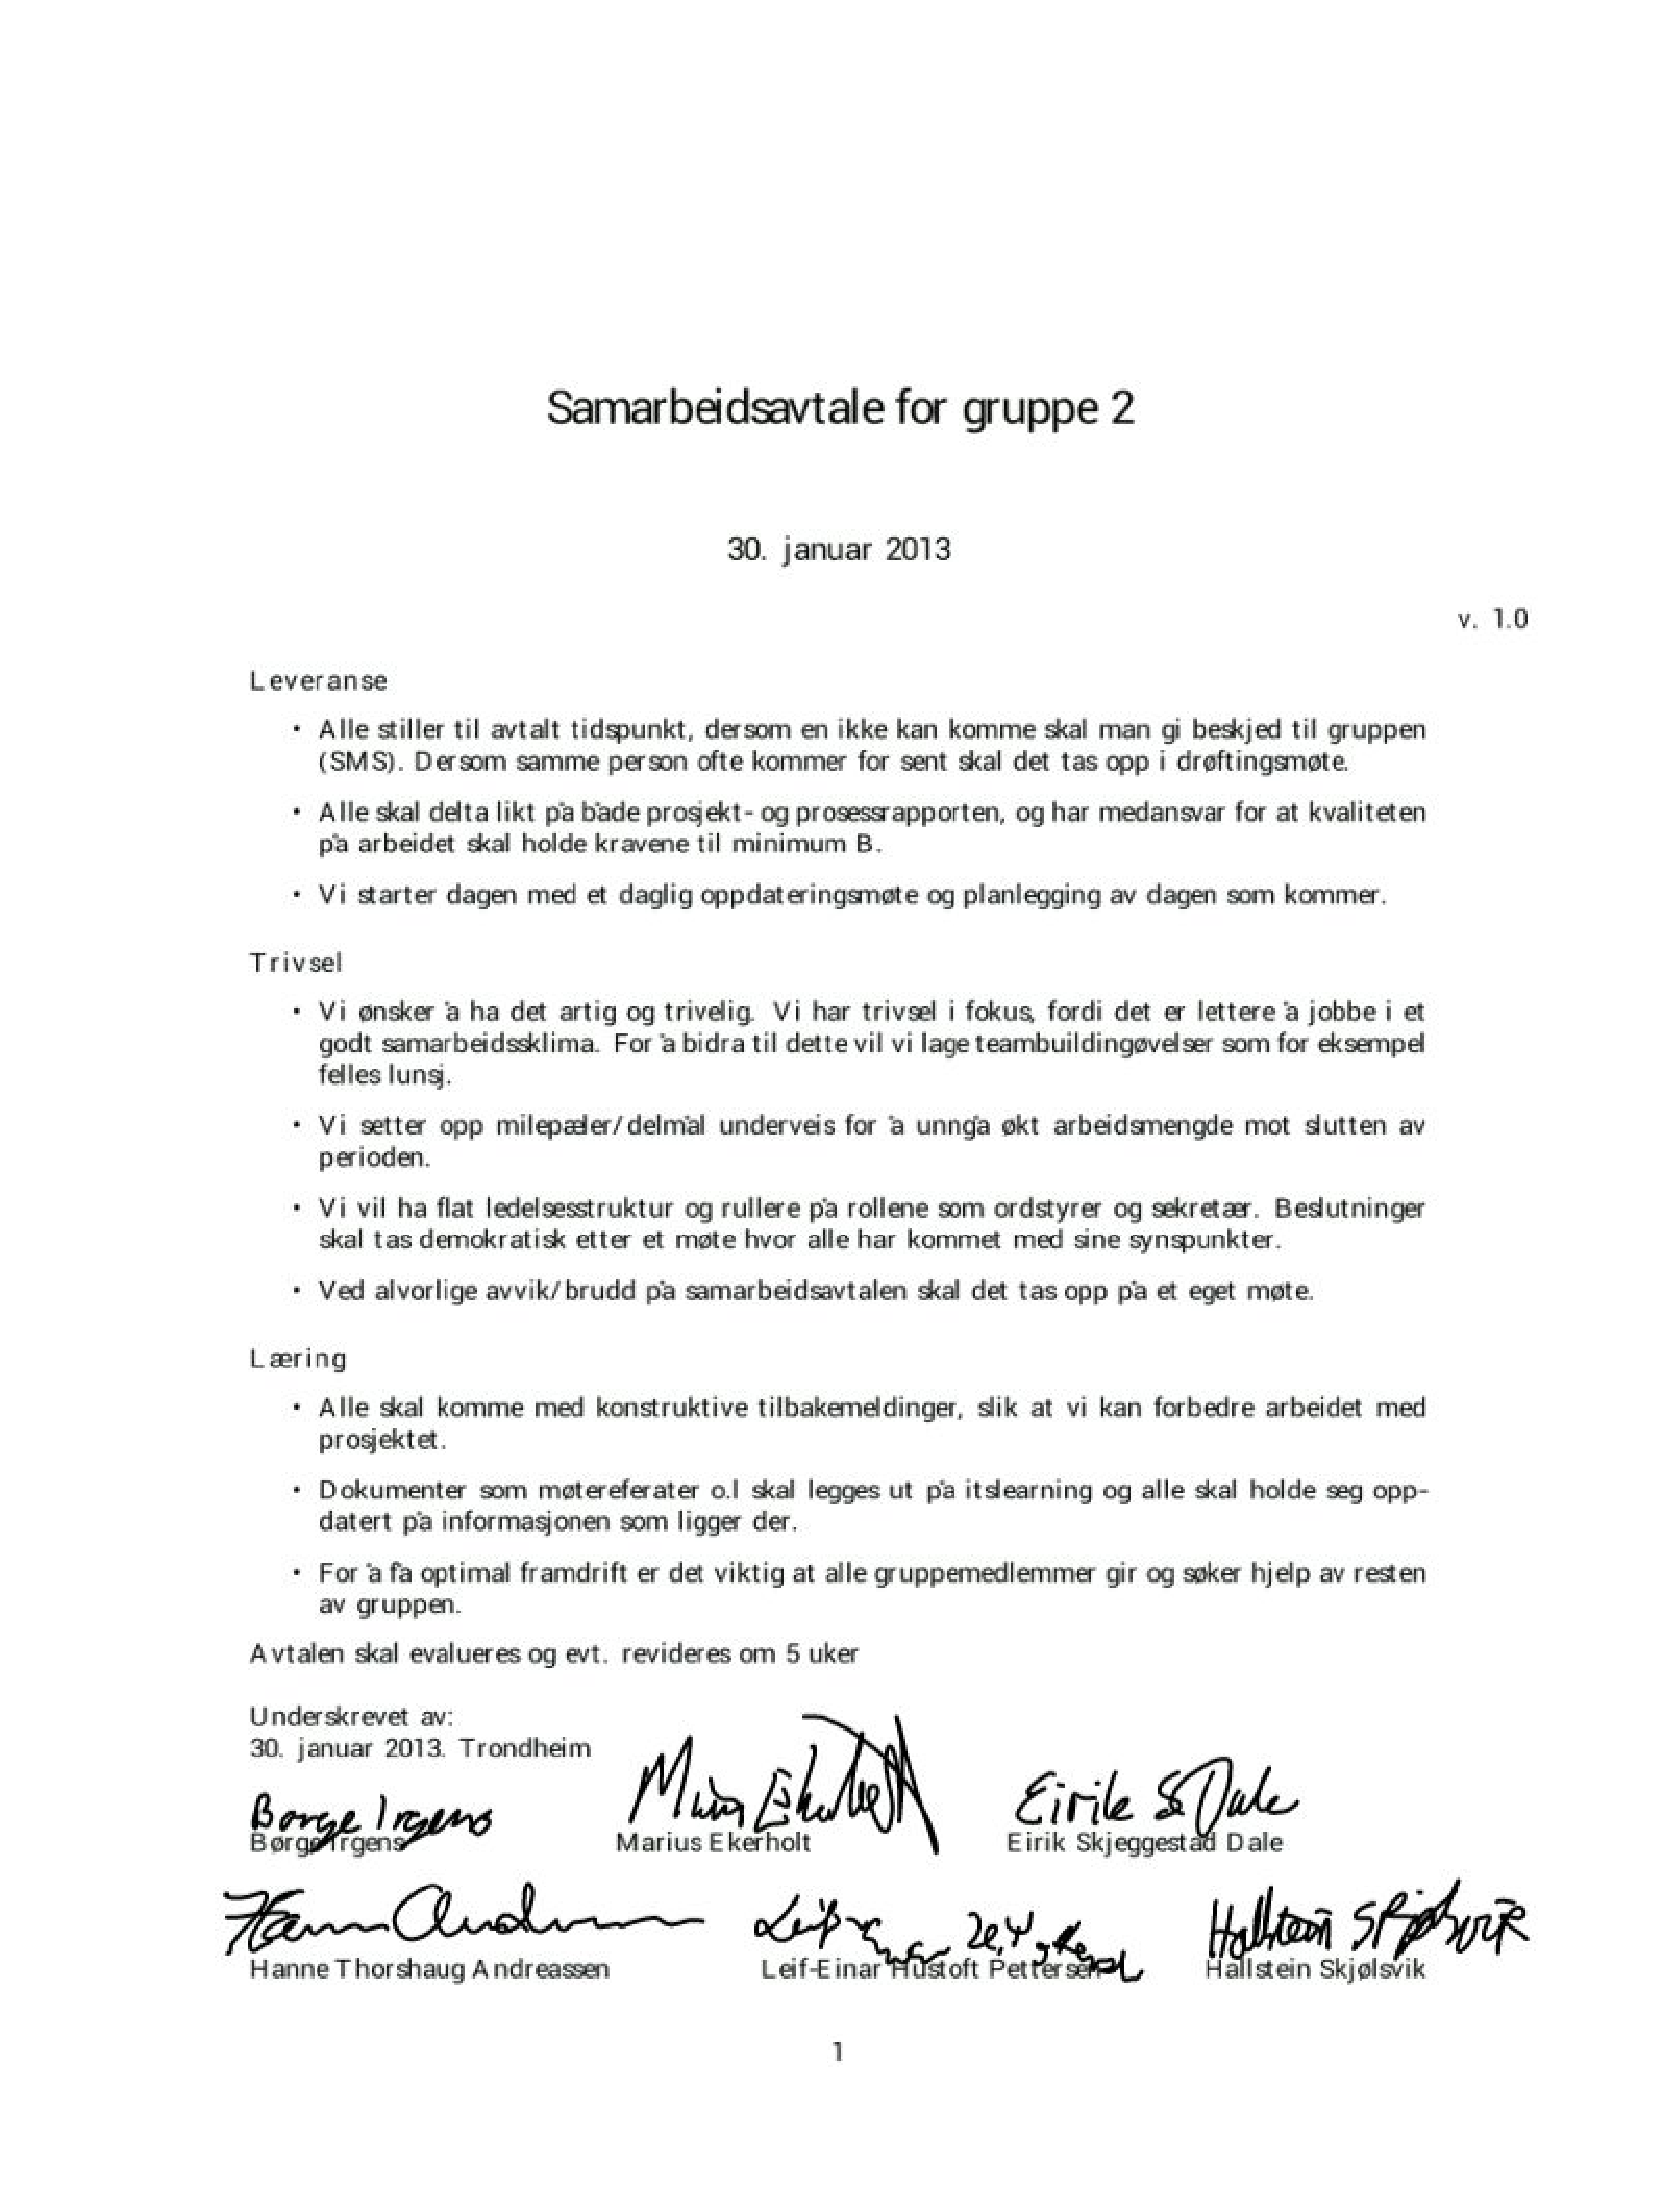
\includepdf[pages={1},pagecommand=\chapter{Teamwork Agreement}\label{teamwork_agreement}]{Figures/teamworkagreement}
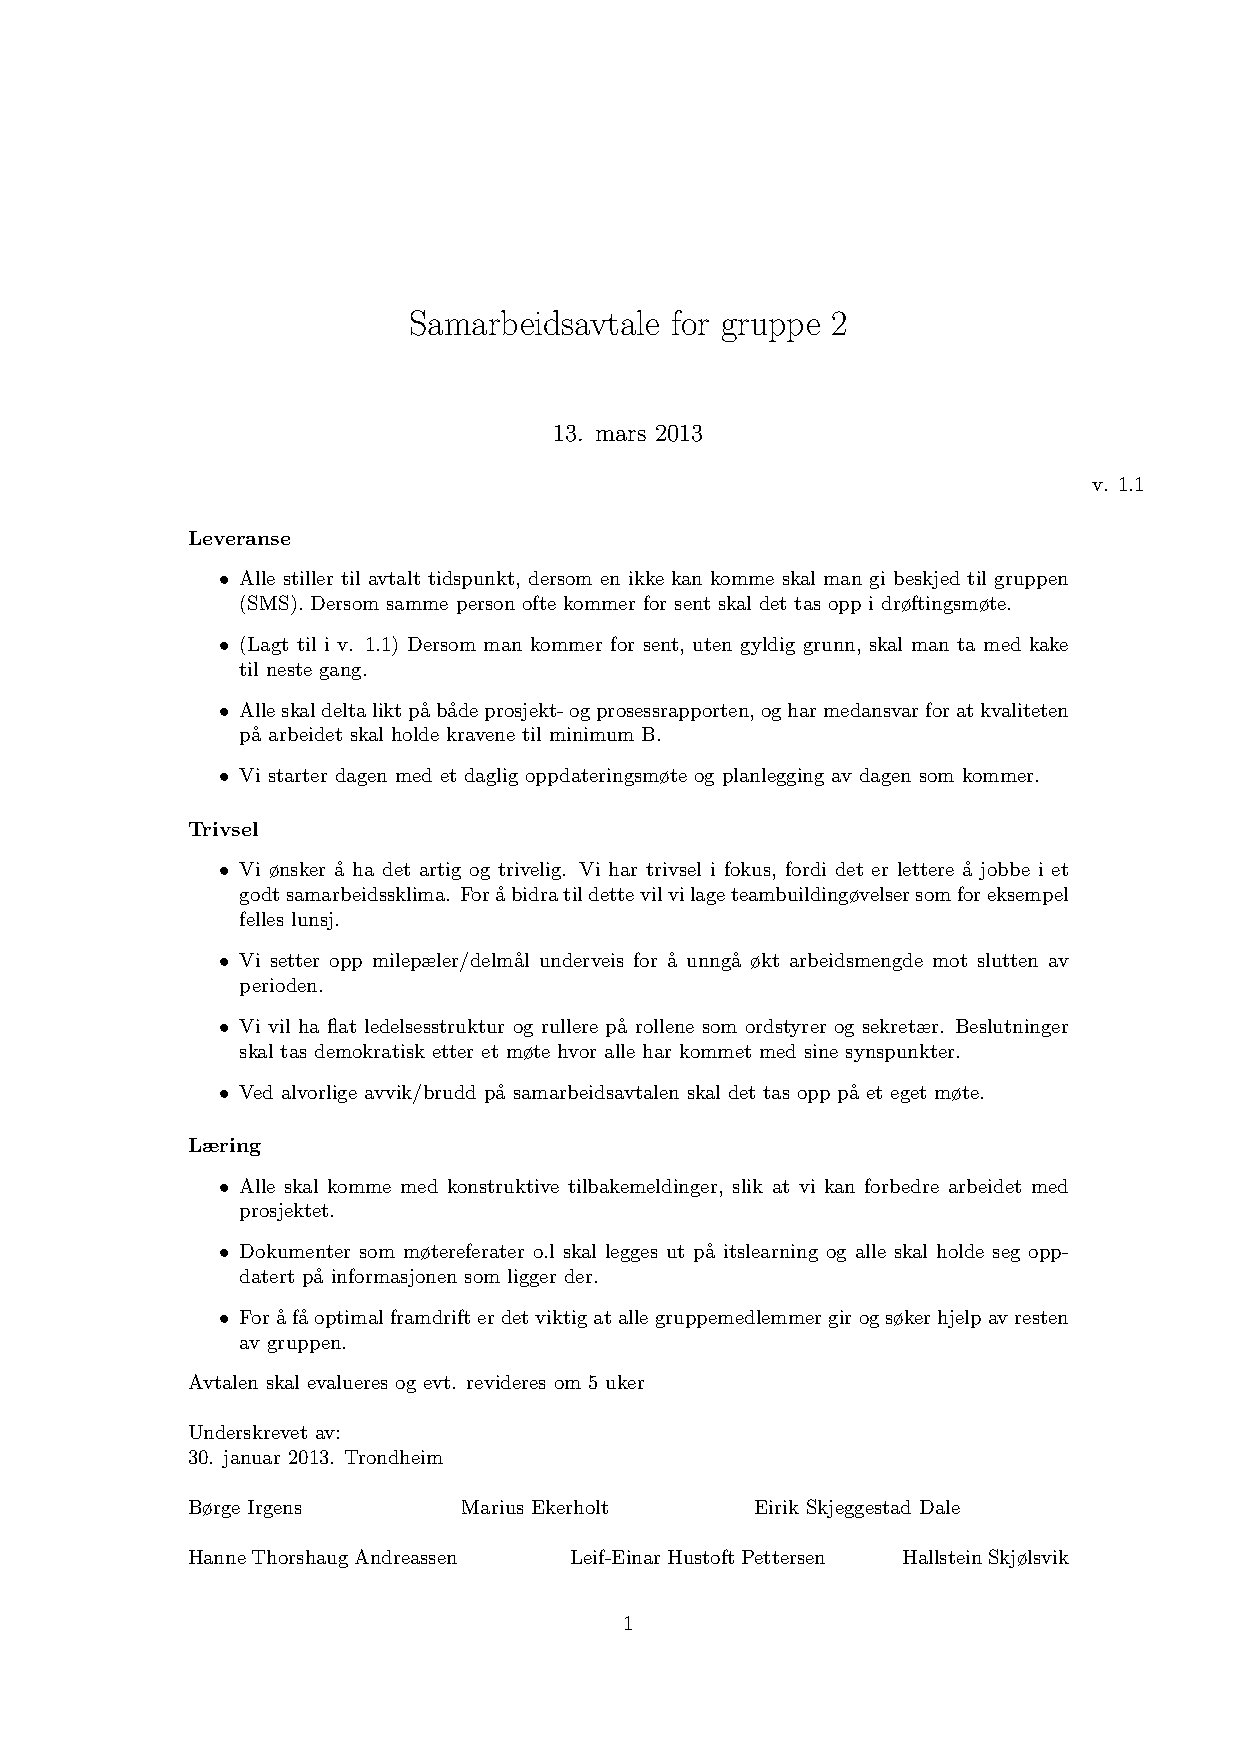
\includepdf[pages={1}]{Figures/newteamworkagreement}

\section{SITRA-exercise}
One of the first group exercises proposed by the facilitators was the SITRA-exercise. In this exercise we were handed a SITRA-sheet where different aspects where colour coded, and we were to evaluate the previous group reflection based on these colours. The colours helped evaluate the group reflections and give us an idea of where on the grading scale the reflections was, by giving different aspects, as shown in \autoref{fig:sitra}. 

During this exercise the group discovered that we had written our first group reflection chiefly by explaining a situation followed by a reflection, both of them quite short and uninformative. This led to a larger focus on a deeper group reflection, with more theory and action considerations where that was applicable. The group felt that the exercise helped give a more objective view on how to write the group reflections, based on how they would be graded.
\newpage{}
\begin{figure}
	\begin{center}
		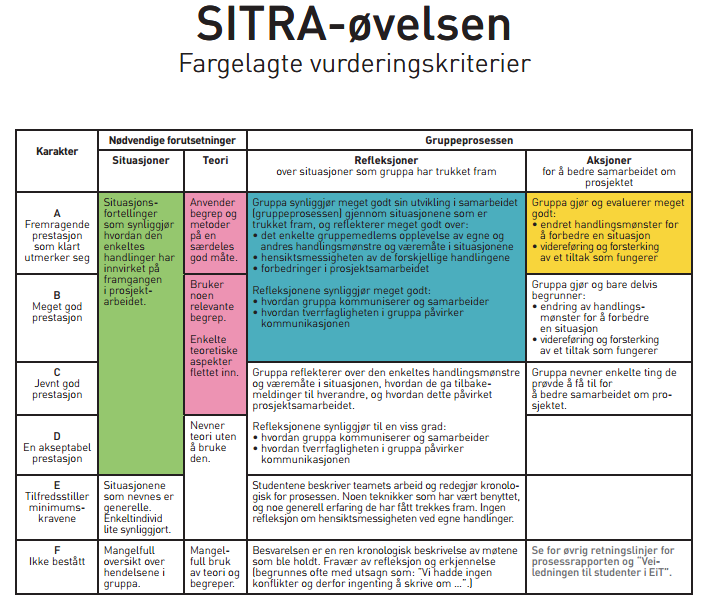
\includegraphics[width=0.7\textwidth]{Figures/sitra.png}
	\end{center}
	\caption[The SITRA Exercise]{The SITRA-sheet given for the SITRA exercise}
	\label{fig:sitra}
\end{figure}
\section{Milestones}
Something about the milestones

% BIBLIOGRAPHY
\begin{thebibliography}{00}
\label{sec:Bibliography}
\bibitem{eksempel-bib-item}{\emph{Navn på item}. October 07 2012. Available at:
	{\tt <}\href{http://www.wikipedia.org/}{www.wikipedia.org}{\tt >}}
\bibitem{aausat3}{\emph{AAUSAT3}. February 13 2013. Available at:
	{\tt <}\href{http://www.space.aau.dk/aausat3/}{http://www.space.aau.dk/aausat3/}{\tt >}}
\bibitem{carpcomm-gs1}{\emph{Carpcomm Ground Station 1}}. October 2012. Available at:
    	{\tt <}\href{ http://carpcomm.com/gs1/}{ http://carpcomm.com/gs1/}{\tt >}
\bibitem{carpcomm-sn}{\emph{Carpcomm Space Network}}. Available at:
     	{\tt <}\href{ http://carpcomm.com/howitworks.html}{  http://carpcomm.com/howitworks.html}{\tt >}
\bibitem{raspberrypi}{\emph{Raspberry pi}}. Available at:
     	{\tt <}\href{ http://www.raspberrypi.org/}{ http://www.raspberrypi.org/}{\tt >}
\bibitem{eks-kom}{Amundsen, Morten et al., Ekstern kommunikasjon, 2011}
\bibitem{GENSO}{\emph{The educational part of ESAs'home page}. Available at:
	{\tt <}\href{http://www.esa.int/Education/Global_Educational_Network_for_Satellite_Operations}{http://www.esa.int/Education/Global_Educational_Network_for_Satellite_Operations}{\tt >}}
\end{thebibliography}


\end{document}
% END DOCUMENT